\documentclass{aastex61}
%Packages
\usepackage{graphicx}
\usepackage{soul, listings, xcolor}
\usepackage{amsmath}
\usepackage{url}
%Code environment details
\definecolor{dkgreen}{rgb}{0,0.6,0}
\definecolor{gray}{rgb}{0.5,0.5,0.5}
\definecolor{mauve}{rgb}{0.58,0,0.82}
\definecolor{grey}{gray}{0.95}
\lstset{frame=tb,
	escapeinside={(*@}{@*)},
	frame = single,
	aboveskip=3mm,
	belowskip=3mm,
	showstringspaces=false,
	columns=flexible,
	basicstyle={\small\ttfamily},
	numbers=none,
	numberstyle=\tiny\color{gray},
	keywordstyle=\color{blue},
	commentstyle=\color{dkgreen},
	stringstyle=\color{mauve},
	breaklines=true,
	breakatwhitespace=true,
}

%% The default is a single spaced, 10 point font, single spaced article.
%% There are 5 other style options available via an optional argument. They
%% can be envoked like this:
%%
%% \documentclass[argument]{aastex61}
%% 
%% where the arguement options are:
%%
%%  twocolumn   : two text columns, 10 point font, single spaced article.
%%                This is the most compact and represent the final published
%%                derived PDF copy of the accepted manuscript from the publisher
%%  manuscript  : one text column, 12 point font, double spaced article.
%%  preprint    : one text column, 12 point font, single spaced article.  
%%  preprint2   : two text columns, 12 point font, single spaced article.
%%  modern      : a stylish, single text column, 12 point font, article with
%% 		  wider left and right margins. This uses the Daniel
%% 		  Foreman-Mackey and David Hogg design.
%%
%% Note that you can submit to the AAS Journals in any of these 6 styles.
%%
%% There are other optional arguments one can envoke to allow other stylistic
%% actions. The available options are:
%%
%%  astrosymb    : Loads Astrosymb font and define \astrocommands. 
%%  tighten      : Makes baselineskip slightly smaller, only works with 
%%                 the twocolumn substyle.
%%  times        : uses times font instead of the default
%%  linenumbers  : turn on lineno package.
%%  trackchanges : required to see the revision mark up and print its output
%%  longauthor   : Do not use the more compressed footnote style (default) for 
%%                 the author/collaboration/affiliations. Instead print all
%%                 affiliation information after each name. Creates a much
%%                 long author list but may be desirable for short author papers
%%
%% these can be used in any combination, e.g.
%%
%% \documentclass[twocolumn,linenumbers,trackchanges]{aastex61}

%% AASTeX v6.* now includes \hyperref support. While we have built in specific
%% defaults into the classfile you can manually override them with the
%% \hypersetup command. For example,
%%
%%\hypersetup{linkcolor=red,citecolor=green,filecolor=cyan,urlcolor=magenta}
%%
%% will change the color of the internal links to red, the links to the
%% bibliography to green, the file links to cyan, and the external links to
%% magenta. Additional information on \hyperref options can be found here:
%% https://www.tug.org/applications/hyperref/manual.html#x1-40003






%% This is the end of the preamble.  Indicate the beginning of the
%% manuscript itself with \begin{document}.

\begin{document}

\title{Lab 1: Exoplanet Transit \\ AST 443: Observational Techniques in Astronomy}

\date{Performed October 7-8, 2016 and Submitted \today}

\author{Joseph Monroy}

\author{Yogesh Mehta}


\begin{abstract}
Our goal for this experiment was to successfully detect a Jupiter-type exoplanet, and from this to see whether it has the known mid-transit time and transit duration. Also, from the depth of the transit we want to get the planet to stellar radius ratio, which would then give us the planet radius. In our experiment we choose to view the star HD 209458 while its planet HD 209458b, also known as Osiris, was transiting. 

We used a 14-inch Meade LX200-ACF telescope at Mt. Stony Brook Observatory to locate HD 209458, and a SBIG STL-1001E CCD camera to measure the flux received before, during and after the transit. Using various Python scripts shown in the Appendix and other astronomy programs, we were able to reduce the data and get a light curve of HD 209458. From this light curve, we deduced that the radius of Osiris is 1.5072 $\pm$ 0.08674 $R_{\text{Jup}}$. 
\end{abstract}

\section{Introduction (JM)} \label{sec:intro}
It has only been within the past decade and a half that we have been able to detect planets around other stars. This has been a major breakthrough in all fields of astronomy because it allows us to see what kind of planets form around different types of stars. Also, it allows us to speculate more on whether we are alone in the universe or not. The most recently discovered method used to detect exoplanets is through transit photometry. This method allows us to point our telescope to a star and see if theres a change in observed flux. Depending on the duration of the observed flux from the star we can determine if there is a transiting body. 

This is the method we used in our experiment and it has proven very successful over the years for hundreds of other astronomers. Although it has already been confirmed that there is an exoplanet around HD 209458, our experiment was significant because it allowed us to see first hand how powerful the method of transit photometry is. By just knowing the dip in relative flux, we can determine the ratio between the radii of the planet and star. Then from knowing the radius of the host star, we can determine the radius of the exoplanet. This is the reason why this method is so powerful: it allows us to learn the properties of planets hundreds of light years away without even viewing or seeing the planet. 

\section{Observations (JM)}
We decided to observe HD 209458 because of the unique characteristics of the system. The star is of G type making it very similar to our own star, having a mass of 1.148 $\pm$ 0.022 $M_\sun$ \citep{2010MNRAS.408.1689S} and a radius of 1.146 $\pm$ 0.050 $R_\sun$ \citep{2001ApJ...552..699B}. The planet has a radius 1.451 times that of Jupiter with an uncertainty of 0.074, while orbiting at nearly one eighth the orbital radius of Mercury to the Sun \citep{2015MNRAS.447..846B}. This makes Osiris a hot Jupiter type planet because its the size of Jupiter but extremely close to it's star. This type of system is a great candidate for exoplanet detection through transit photometry. This is because the star is of average size, while having a huge Jupiter size planet orbiting it. This makes detecting a dip in the relative flux when the planet transits a lot easier. The only negative about this system is the orbital radius of Osiris, because the closer a planet is to its star the harder it will be to detect it. Although it makes up for it by the size of Osiris and the relatively bright star of 7.65 apparent magnitude.

We were able to observe HD 209458 and its transiting planet by using a 14-inch Meade LX200-ACF telescope with a SBIG STL-1001E CCD camera attached. This yields a field of view of 26 arcminutes for the exposures. All observations were held at the Mt. Stony Brook Observatory. The weather that night was mostly clear with some thin, high-altitude clouds in the beginning of observations. By the end of the experiment the sky was largely clear of clouds. The seeing was mostly good throughout the night as well, with there being very little wind. We calculated the total transit duration to be 3.024288 hours, with a mid-transit time of October $8^{\text{th}}$, 2016 at 03:11 UTC. The transit duration was calculated using the following equation:
\begin{equation}
T_{\text{duration}} = \frac{P}{\pi}\arcsin\left(\frac{\sqrt{(R_*+R_P)^{2}-(bR_*)^{2}}}{a}\right)
\end{equation}
Where $P$, $a$ and $b$ are all the period, semi-major axis and impact parameter of the planet respectively, and $R_*$ and $R_P$ are the radii of the star and planet respectively. The impact parameter is given by:
\begin{equation}
	b = \frac{a \cos(i)}{R_*}
\end{equation}
Where $i$ is the inclination angle of the planets orbit. In this case, the semi-major axis, inclination angle and period of HD 209458 b are 0.04747 AU, 86.59 degrees and 3.52472 days respectively. All these values are from the The Extrasolar
Planets Encyclopedia \footnote{\url{http://exoplanet.eu/catalog/hd_209458_b/}}. The mid-transit time was calculated from knowing the period of the planet, and knowing a specific time when the transit began in the past. From this information we simply just have to keep adding the period time to the time of transit until we reach current day. We figured out where our star should be in the night sky by using the program StarAlt. It helps show whether stars are viewable depending on your location on Earth and your elevation.

We first tried to find the star by going to its right accession and declination, and made sure that the star we found was HD 209458 by looking at our finder charts. Once we confirmed the star we made sure it was centered on the cross hairs of the eyepiece. We then made sure the CCD camera was connected correctly to the telescope and the program CCDSoft, which is used for adjusting the exposure times and other settings of the CCD. We first tried to take four exposures of our star with an exposure time (exp. time) of three seconds each. This resulted in counts that were too high because the star was focused too well on the CCDSoft. High counts are bad because the pixels on the CCD can be oversaturated at around 60,000 counts and not yield good data. So for the next exposure we defocused the star, while increasing the exposure time to five seconds, which resulted in lower counts around 20,000. We kept this exposure time for the rest of the science exposures. By the end of the experiment we took 1,461 science exposures, all with an exposure time of five seconds. After this we started to take our calibration data, starting with the darks. In order to take the darks we put the telescope cap back on so we have complete darkness. We then took 19 dark exposures each of five seconds, then we took out flats. We took the cap off and pointed the telescope towards a equally lit part of the dome. At first we took 19 flats each of five seconds, but it turned out the counts were too high. So we lowered the exposure time to three seconds and lowered the lights in the observatory. This yielded in lower counts and better flat fields. Finally we took another set of flats with a shorter exposure time of one second. This is so later we can create a bad pixel mask so we know where the bad pixels are on the CCD. Below is a table of the logsheet we used during observations. The time written down is in EST, and was taken from the computer we were using. 
\begin{deluxetable*}{ccCrlc}[h!]
	\tablecaption{Logsheet of Observations \label{tab:logsheet}}
	\tablecolumns{13}
	\tablenum{1}
	\tablewidth{0pt}
	\tablehead{
		\colhead{File Number} &
		\colhead{Object} &
		\colhead{Exp. Time} & \colhead{Time} & \colhead{Comments} \\
		\colhead{} & \colhead{} & \colhead{(s)} & \colhead{(EST)} & \colhead{}
	}
	\startdata
	science.0-4 & transit & 3 & 8:41 pm & Focused too well \\
	science.5 & $\downarrow$ & 5 & 8:42 pm & Max. count of 23,000 \\
	science.6 & $\downarrow$ & $\downarrow$ & 8:43 pm & First of 800 \\
	science.7-75 & $\downarrow$ & $\downarrow$ & 8:55 pm & \nodata \\
	science.76-797 & $\downarrow$ & $\downarrow$ & 10:55 pm & Last of 800 set \\
	science.798 & $\downarrow$ & $\downarrow$ & 10:55 pm & First of next 800 \\
	science.1087-1088 & $\downarrow$ & $\downarrow$ & 11:42 pm & Long streak of light appeared \\
	science.1461 & transit & $\downarrow$ & 12:43 am & Last transit exposure \\
	darks.0-19 & darks & $\downarrow$ & 12:58 am & 19 darks taken \\
	flats.0-19 & flats & 5 & 1:05 am & Exposures was too long \\ 
	flats.20-29 & $\downarrow$ & 3 & 1:07 am & Lowered lights and exposure, counts at 18,000 \\
	flats.30-39 & $\downarrow$ & 1 & 1:08 am & Shorter exposure, counts at 6,000 \\
	\enddata
\end{deluxetable*}

\section{Data Reduction (JM and YM)}
The data we obtained from all the exposures were in the form of raw .FIT files. So in order to make the science .FIT files usable we needed to create a Master Flat field, a Master Dark field and a bad pixel mask from all the calibration data. The master dark image was used to correct for the dark current and the master flat field was used to scale each pixel by its sensitivity relative to the other pixels on the CCD. The bad pixel mask found any pixels with a response that was nonlinear in time. If the pixels are linear, the ratio of the counts from the long exposure flats to those of the short exposures should equal the ratio of the time of the long exposure to that of the short. Any pixel that deviated from this was deemed "bad." The ratio of the times is 3. This was all done using the Python code from appendix \ref{code: reduction}, which created clean science images. We found two bad pixels. Ordinarily, we would have taken an average of the surrounding pixels to extrapolate what the each bad pixel should have given us. However, since these pixels were in areas of the field that were never used, we simply ignored any information from them. All of the data reduction was done through the uhura astronomy computer using a secure shell client. 

When we performed the experiment, the auto-guider on the telescope did not work, so we had to use the astronometry.net software to get the position and coordinates of all the stars in our .FIT files. We wrote a script to let the software run through all of our images. Next, we used the program Source Extractor to return the properties of all the stars in our images, most importantly the relative flux. However, we needed to know the aperture size Source Extractor should use to get the data from the stars. This could be found out by opening up one of our clean images in ds9 and seeing what the radius in pixels is of our target star. Although this aperture is larger than what we would like to maximize the signal to noise ratio, the larger size reduces the effects of seeing. Once we found this radius, we inputed it into the Source Extractor configuration file and obtained the properties of every object in all of our images. We once again wrote a script that runs all our images through Source Extractor. All of the code for this part can be found in appendix \ref{code: astro sex}.

We finally now had the three properties we need to get our analyzed data: the time of each image, flux received from all the stars in one image, and the error in that flux. Next, we chose ten reference stars in our clean images and took their respective times, flux, and the error in the flux from the table. We did this because it allows us to calibrate the flux received from the target star, correcting for changes in the atmosphere, seeing, and airmass. All of these stars have similar brightness when we viewed them in ds9. We used the code from appendix \ref{code: flux} to find our stars in each image and get their fluxes and errors in each exposure. 

Unfortunately, our code would sometimes match to the wrong star in an exposure, resulting in an outlier in our lightcurves. This would not happen for any particular exposure or star. Although it was applied randomly, it was consistent. It would mismatch a particular star for a particular image the same way every time it ran. This might indicate a problem with the code's logic, but the fact that it wouldn't affect every star in the same place or with the same frequency indicates otherwise. There were no syntactic errors. We even made sure all of the indents were spaces instead of a mix of spaces and tabs. Another possibility was that astronometry.net was not solving our fields properly. To address this, we opened up an image with an outlier for a particular star and 3 images that were matched correctly for the same star. We locked their WCS coordinates and had them disappear and reappear on top of each other. This would let us see if the whole image would shift because astronometry gave it a wrong WCS coordinate. There was no observed shift. Unable to find the cause, we set the flux for the stars to zero for every exposure in which the star was mismatched. 

From the fluxes of each reference star, we rescaled them to by the star's average flux over all exposures taken. This was done also to the error in the flux, shown in \eqref{eq: norm}, where $f_{j}(t)$ is the flux for some reference $j$ at time $t$ and $\sigma_{f_{j}(t)}$ is the error in that particular flux.
\begin{equation} \label{eq: norm}
f_{j}(t)  \rightarrow \frac{f_{j}(t)}{\langle f_{j} \rangle}       \;\;\;\;\;\;\;\sigma_{f_{j}(t)} \rightarrow \frac{\sigma_{f_{j}(t)}}{\langle f_{j} \rangle}
\end{equation}
We normalized the flux and its error because it would allow us to visualize any environmental changes that occurred throughout the night, as well as the overall shape of the lightcurves for each star. Once we had this, we plotted each of the stars' flux as a function of time. The time is the number of seconds after midnight on October $8^{\text{th}}$ in UTC time. Although the averages did take into account the non-mismatched outliers of each star, they were so few in number that the average remained unperturbed. These are shown in Fig. \ref{fig: refcurve1} - \ref{fig: scicurve1}. This was done with the code from appendix \ref{code: curves}. 
%Light Curves
\begin{figure}[hbt!]
	\centering
	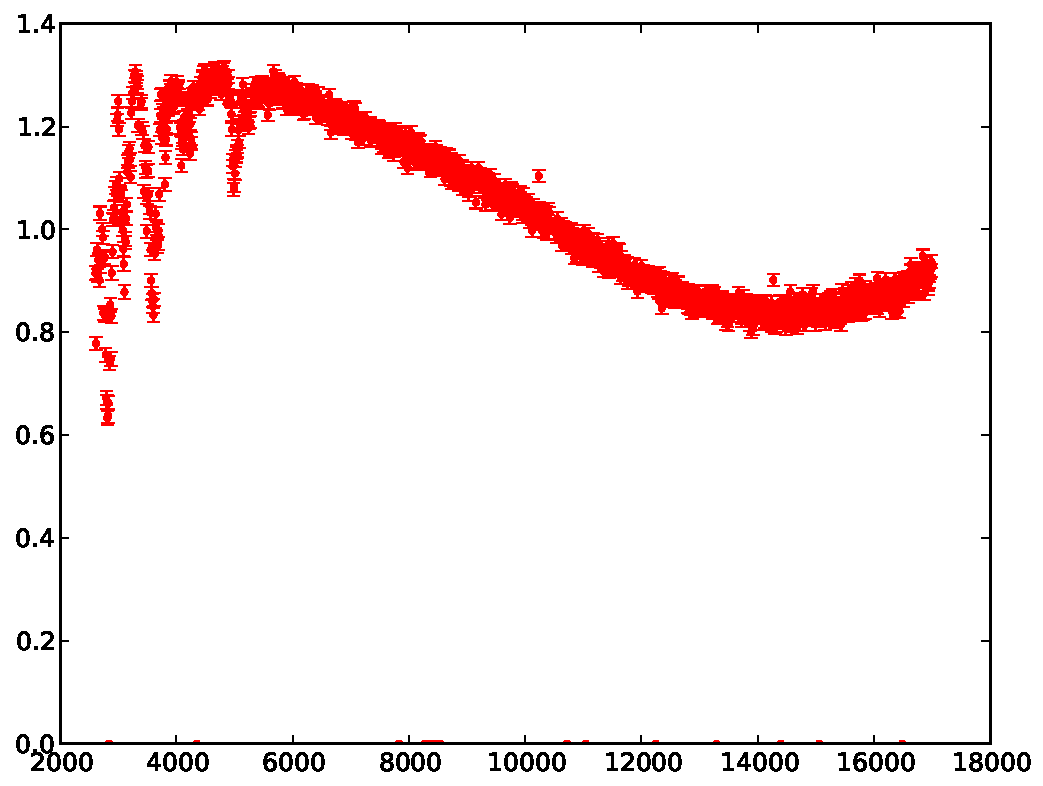
\includegraphics[scale = .45]{exo_curves1.pdf}
    \caption{Reference star 1. This variable star was removed for the duration of the experiment}
    \label{fig: refcurve1}
\end{figure}
\begin{figure}[hbt!]
	\centering
	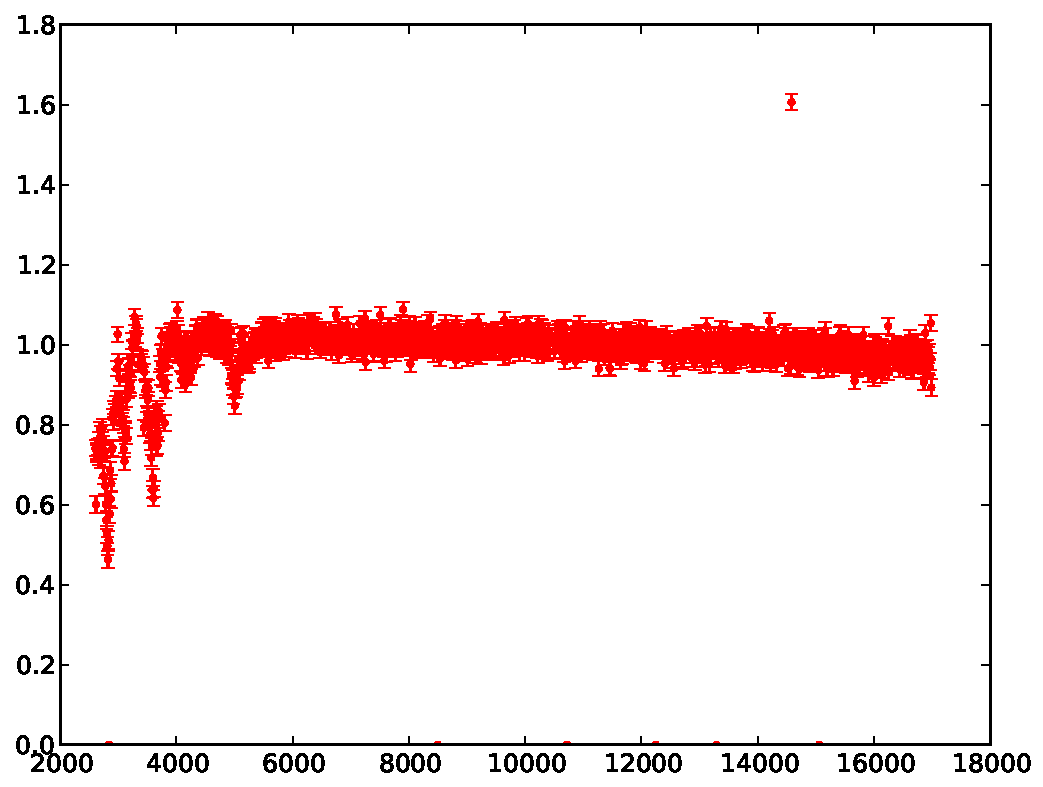
\includegraphics[scale = .45]{exo_curves2.pdf}
	\caption{Reference star 2}
	\label{fig: refcurve2}
\end{figure}
\begin{figure}[h]
	\centering
	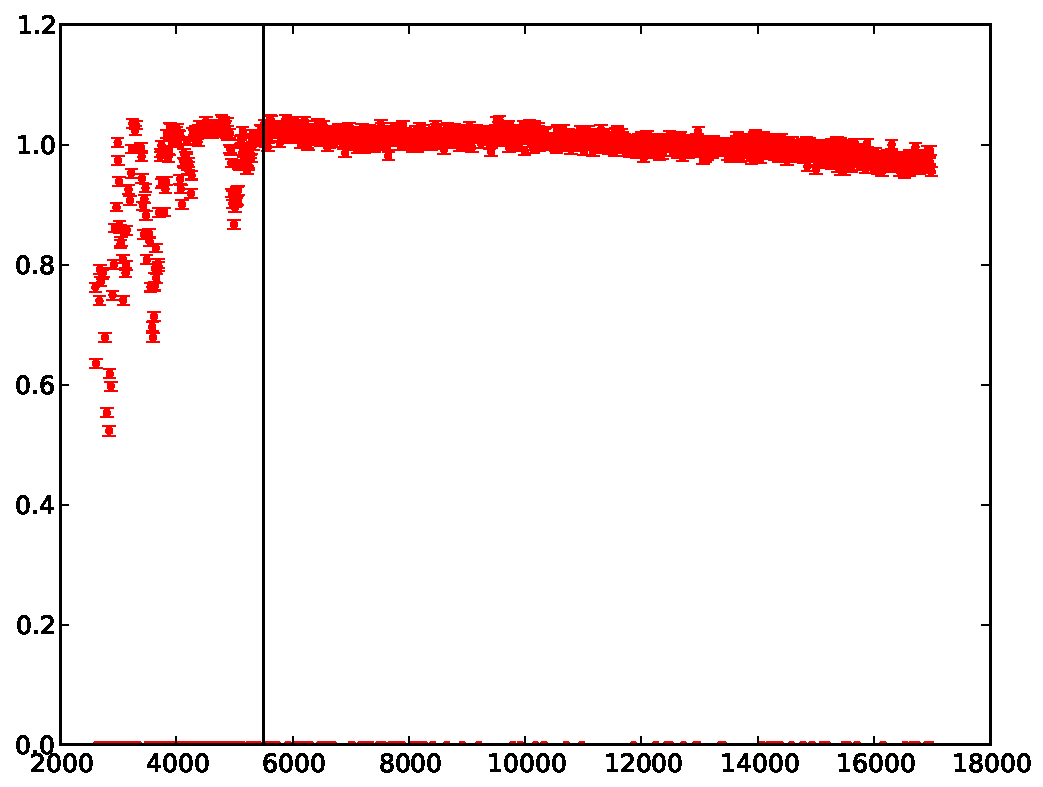
\includegraphics[scale = .45]{exo_curves3.pdf}
	\caption{Reference star 3}
	\label{fig: refcurve3}
\end{figure}
\begin{figure}[h]
	\centering
	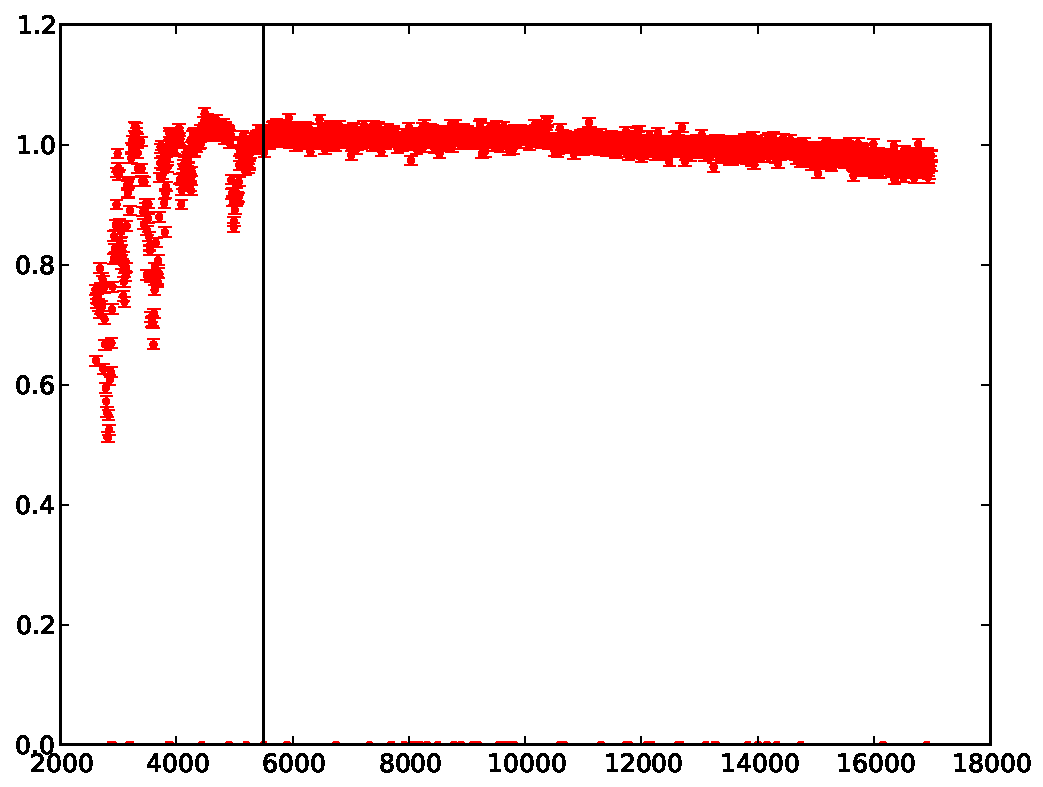
\includegraphics[scale = .45]{exo_curves4.pdf}
	\caption{Reference star 4}
	\label{fig: refcurve4}
\end{figure}
\begin{figure}[h]
	\centering
	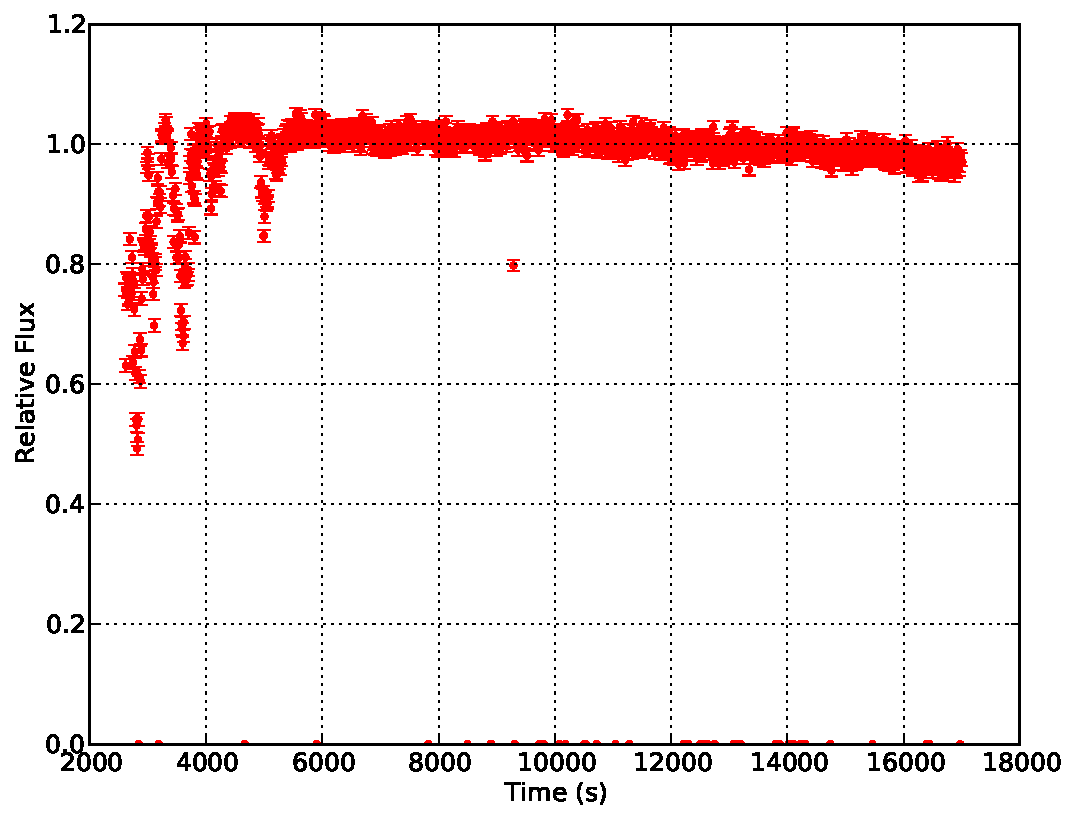
\includegraphics[scale = .45]{exo_curves5.pdf}
	\caption{Reference star 5}
	\label{fig: refcurve5}
\end{figure}
\begin{figure}[h]
	\centering
	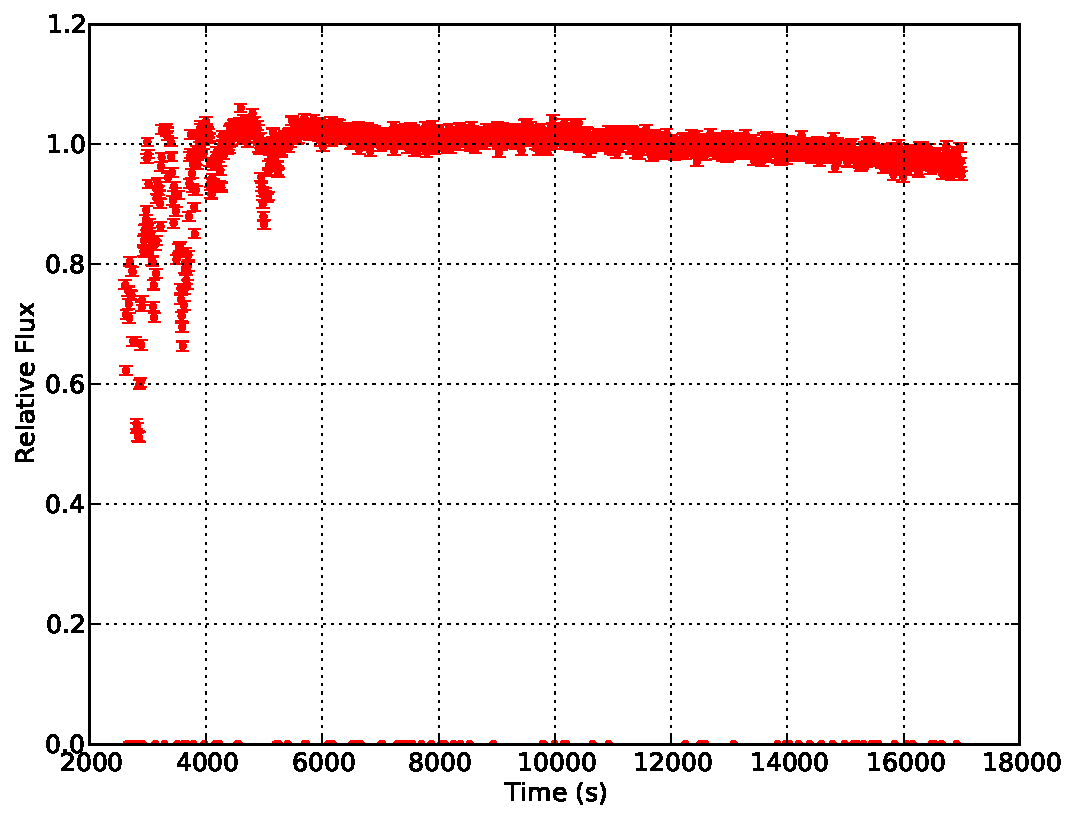
\includegraphics[scale = .45]{exo_curves6.pdf}
	\caption{Reference star 6}
	\label{fig: refcurve6}
\end{figure}
\begin{figure}[h]
	\centering
	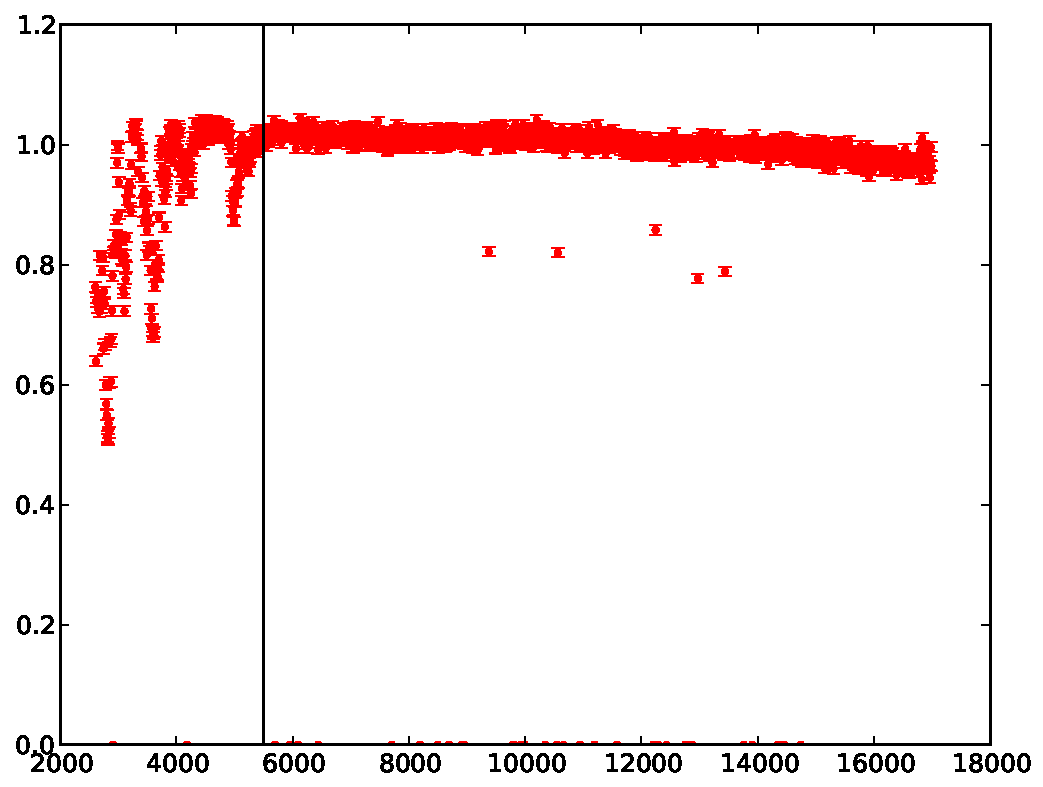
\includegraphics[scale = .45]{exo_curves7.pdf}
	\caption{Reference star 7}
	\label{fig: refcurve7}
\end{figure}
\begin{figure}[h]
	\centering
	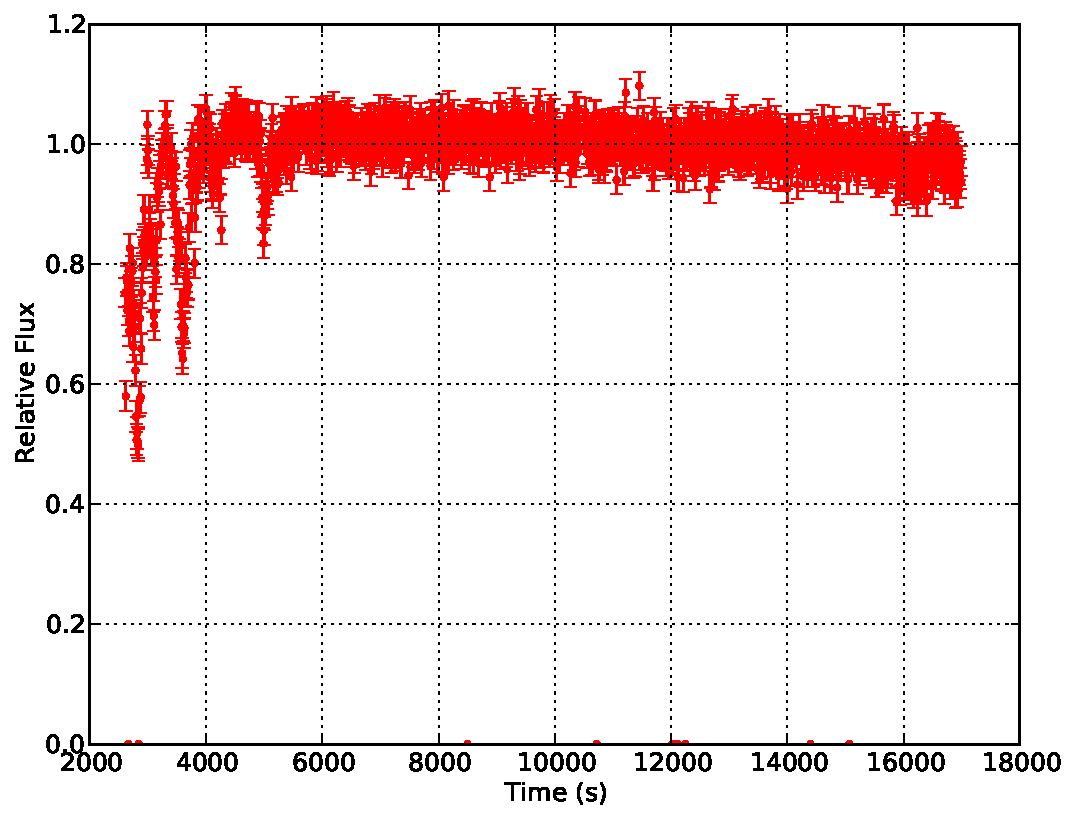
\includegraphics[scale = .45]{exo_curves8.pdf}
	\caption{Reference star 8}
	\label{fig: refcurve8}
\end{figure}
\begin{figure}[h]
	\centering
	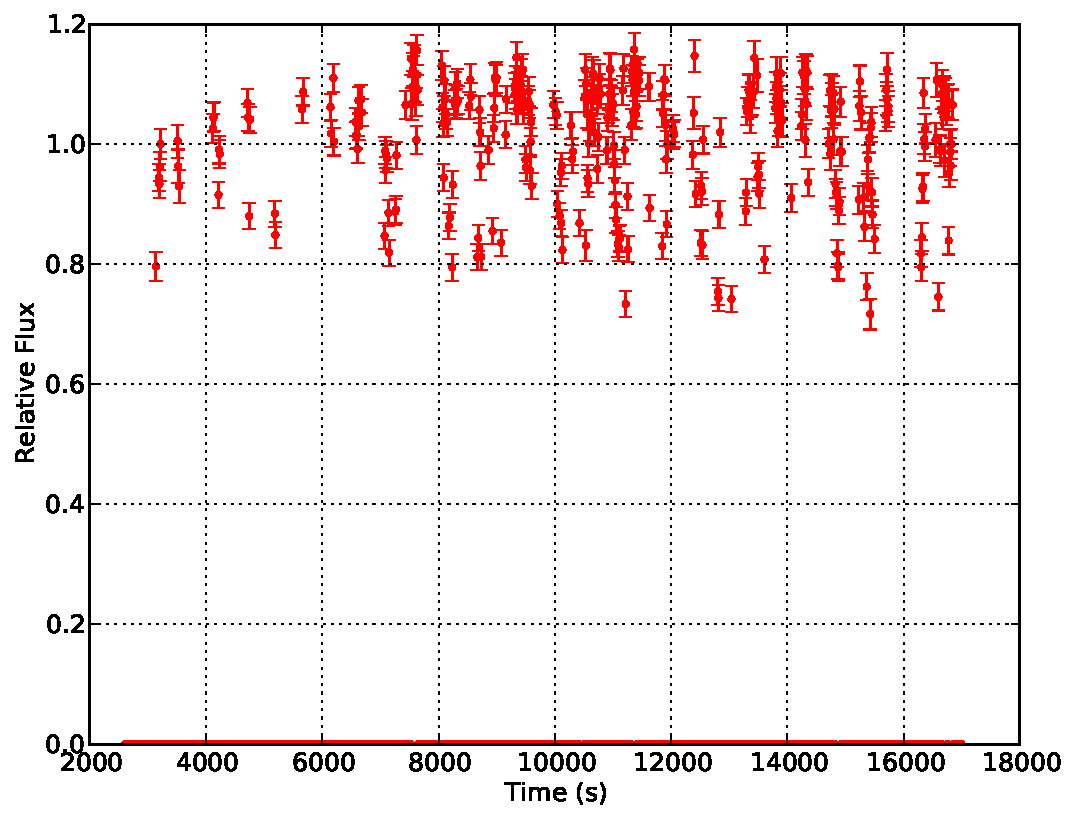
\includegraphics[scale = .45]{exo_curves9.pdf}
	\caption{Reference star 9. The outliers rendered this star useless.}
	\label{fig: refcurve9}
\end{figure}
\begin{figure}[h]
	\centering
	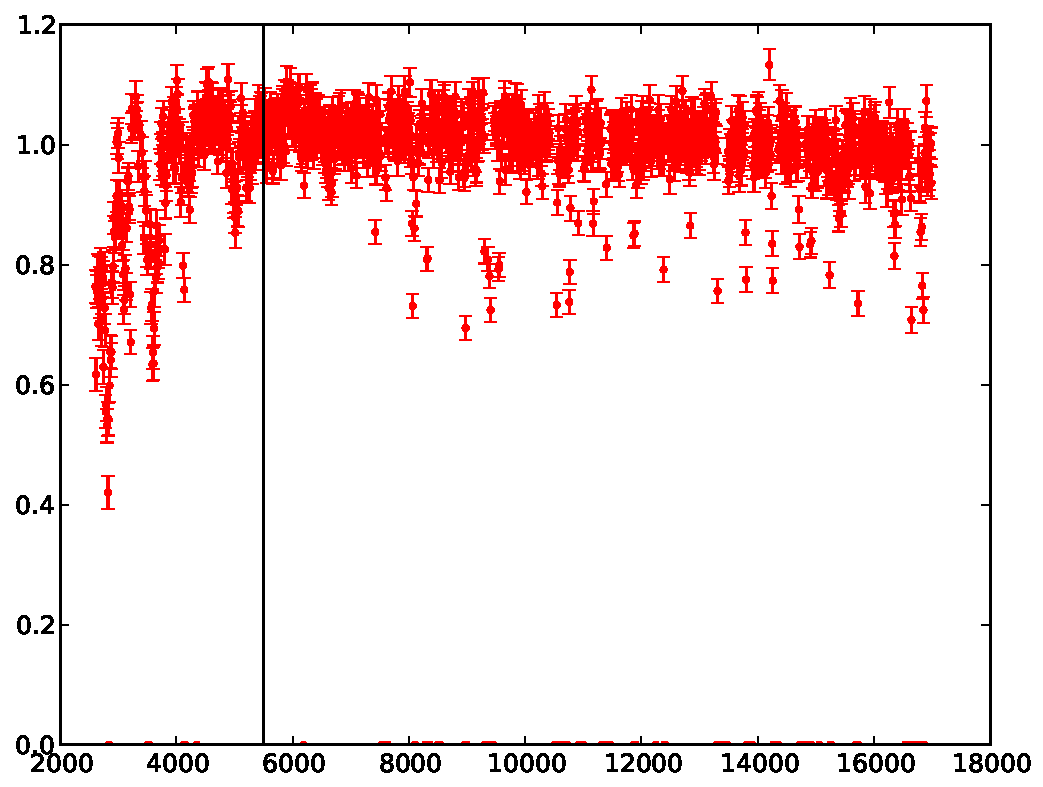
\includegraphics[scale = .45]{exo_curves10.pdf}
	\caption{Reference star 10. This star was scrapped because of its outliers and large spread}
	\label{fig: refcurve10}
\end{figure}
\begin{figure}[h]
	\centering
	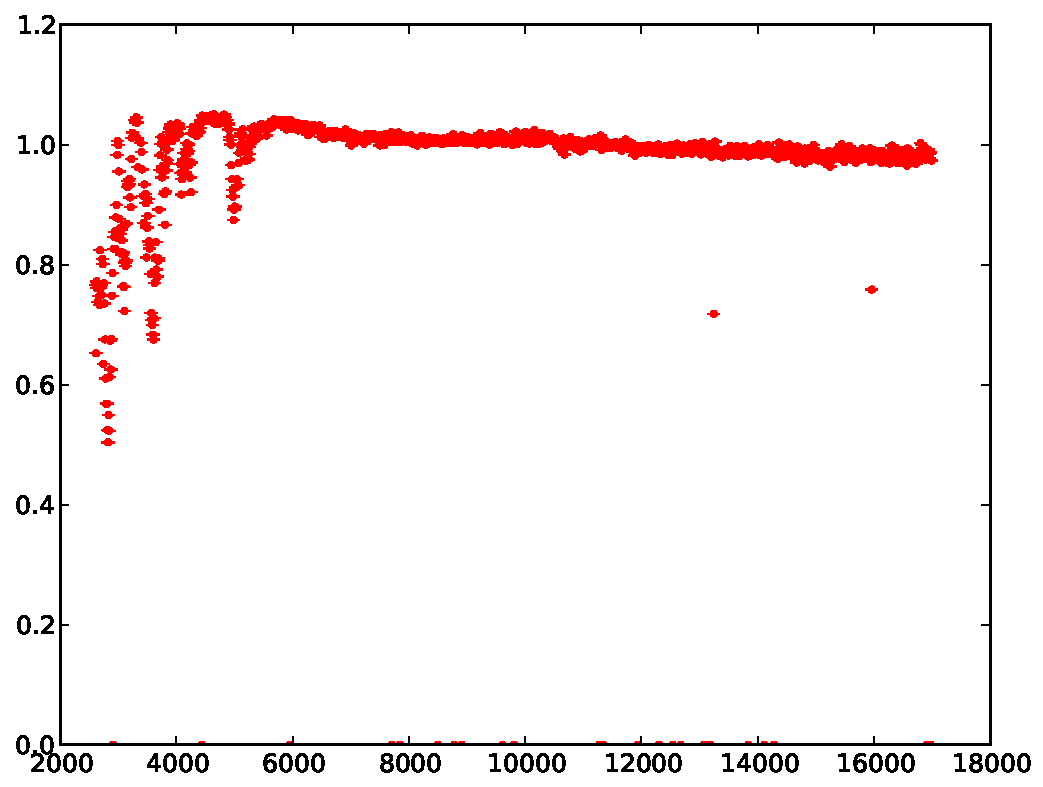
\includegraphics[scale = .45]{exo_curves11.pdf}
	\caption{Normalized light curve of science target}
	\label{fig: scicurve1}
\end{figure}

From these curves we can see vast changes in flux caused by the atmospheric conditions early that night. Due to this much variability, these images were not factored into the normalization of the plots. The normalization also ignored the fluxes at zero, which correspond to the mismatched outliers. The remaining outliers were removed via sigma clipping. Any value more than 4 sigma off from the average was removed for the duration of the experiment.

Based on the lightcurves, we had to remove some reference stars entirely. The first of these, shown in Fig. \ref{fig: refcurve1}, is a variable star. Its intrinsic flux variations would throw off our calibration, making it seem as though there were atmospheric changes where there were none. Another reject is the ninth reference star, seen in Fig. \ref{fig: refcurve9}. This star appears to have been mismatched more often than not. Combining that with the large spread on the correctly matched fluxes and it becomes unusable. The final star we had to scrap was the tenth reference star, found in Fig. \ref{fig: refcurve10}. This was because of the unusually large spread and high number of correctly matched outliers.

Now that we have our reference stars, we can account for environmental influences on the flux from the target star by calculating it relative to the flux of the reference stars. In order to get all the flux from all the reference stars we need to calculate the weighted mean in each clean image. This can be found by using \eqref{eq: average}, where $\mu_{i}^{ref}$ is the weighted mean for any image $i$. This average also has an error, given by \eqref{eq: error}. 
\begin{equation} \label{eq: average}
	\mu_{i}^{ref} = \frac{\sum_{j}\left( \frac{f_{j}^{ref}}{\left( \sigma_{j}^{ref}\right) ^{2}}\right) }{\sum_{j}\left( \frac{1}{\left( \sigma_{j}^{ref}\right) ^{2}}\right) }
\end{equation}
\begin{equation} \label{eq: error}
	\sigma_{i}^{ref} = \sqrt{\frac{1}{\sum_{j}\left( \frac{1}{\left( \sigma_{j}^{ref}\right) ^{2}}\right)}}
\end{equation}
Now that we have the weighted mean of the reference stars, we can get rid of the atmospheric changes in the science images by getting the ratio: $r_{i} = \frac{f_{i}^{sci}}{\mu_{i}^{ref}}$. The error in this ratio is given by Eq. \eqref{error: ratio}. 
\begin{equation}\label{error: ratio}
\sigma_{r_{i}} = r_{i} \sqrt{\left( \frac{\sigma_{f_{i}^{sci}}}{f_{i}^{sci}}\right) ^{2} + \left( \frac{\sigma_{i}^{ref}}{\mu_{i}^{ref}}\right) ^{2}}
\end{equation}
This as all done by the code in appendix \ref{code: bigtable}.

We now have all the information needed: the time, science flux, weighted mean and the ratio of the two latter. The last step involves normalizing the ratio by the baseline flux of our target star (the flux when the planet is not transiting). The baseline flux was calculated by looking at the clean images taken before transiting occurred, and taking the average flux of those images. Since it was so noisy, we only used the exposures from 4000-6000 seconds. The new ratio and its error will then be given by Eq. \eqref{eq: baseline}, where $f_{\text{blf}}$ is the baseline flux for a given star.
\begin{equation}\label{eq: baseline}
r_{i} \rightarrow \frac{r_{i}}{f_{\text{blf}}} \;\;\;\;\;\;\;\;\;\;\; \sigma_{ f_{\text{blf}}} \rightarrow f_{\text{blf}} \sqrt{\left( \frac{\sigma_{ f_{\text{blf}}}}{f_{\text{blf}}}\right) ^{2} + \left( \frac{\sigma_{ r_{i}}}{r_{i}}\right) ^{2}}
\end{equation}

We then binned this normalized data into intervals of 12 images. Since each exposure was 5 seconds, and there was about 4-5 seconds of processing time between exposures, this corresponds to about 2 minutes. This lightcurve is shown in Fig. \ref{fig: lightcurve}.

%Final Lightcurve
\begin{figure}[hbt!]
	\centering
	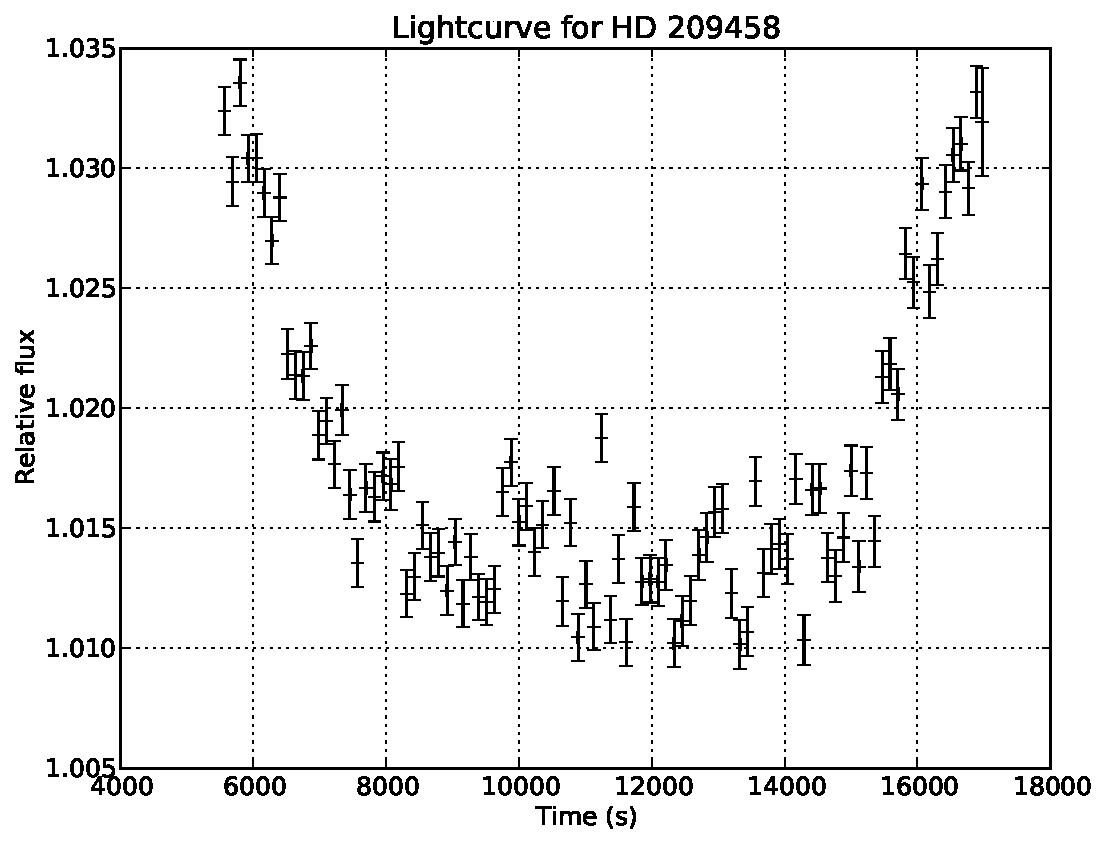
\includegraphics[scale = .75]{exo_lightcurve.pdf}
	\caption{Exoplanet transit. The lightcurve was binned in intervals of about 2 minutes}
	\label{fig: lightcurve}
\end{figure}


\section{Data Analysis and Results (JM and YM)}
We finally reduced all our data to produce a finished light curve of HD 209458b transiting its host star. Now our goal is to determine the radius of the transiting exoplanet. This can be done by first noticing the change in flux based on the transit depth. When the planet is not transiting we should expect to see that the normalized ratio $r_{i}$ should be around 1.0 since we normalized it by the baseline flux. When the transit is occurring we should expect the ratio to be 1.0 - $\epsilon$ , where $\epsilon$ is lowest flux received during the transit. We see that the ratio between the flux during the transit to the flux before is equal to $1-\epsilon$, since the flux before is normalized to 1. We call this quantity $\Delta f$, or the total transit depth. From this, we can get the ratio of the areas between the planet and star. Since we are assuming we are looking at the transit head on, we can assume that both objects are flat disks of area $\pi r^{2}$, where $r$ is the radius of the object. Setting it all up, we have the equation:
\begin{equation}
	\Delta f = \frac{\pi R_{P}^{2}}{\pi R_{*}^{2}}
\end{equation}
Solving for the planet radius we get:
\begin{equation}
	R_{P} = \sqrt{\Delta f \; R_{*}^{2}}
\end{equation}
The error in the radius is given by:
\begin{equation}
	\sigma_{R_{P}} = \frac{R_{P}}{2}\sqrt{\left( \frac{\sigma_{ \Delta f}}{\Delta f}\right)^{2}  + 4\left( \frac{\sigma_{ R_{*}}}{R_{*}}\right)^{2} } 
\end{equation}

Now that we have all the equations set up, we can plug in our values. Looking at the light curve, it can be seen that near the middle of the transit the fluxes get very messy. In order to get a value for the lowest flux in the transit, we took the median of the values from 8,000 to 14,000 seconds. We chose the median over the average as the former is more insensitive to outliers. The error in this is the median absolute deviation, as shown in Eq. \eqref{error: mad}. Here, $f_i$ is the flux at a specific point.
\begin{equation} \label{error: mad}
	\sigma_{\Delta f} = \text{median}(\lvert \Delta f - f_i \rvert)
\end{equation}

This resulted in a value of 0.9809 $\pm$ 0.00136. This yields a transit depth of 0.0190875 $\pm$ 0.0013581. As stated in the Observations section, we have a stellar radius of 1.146 $\pm$ 0.050 $R_{\sun}$. Plugging the values into equations (8) and (9) and converting to $R_{\text{Jup}}$, we get a planet radius of 1.541 $\pm$ 0.087 $R_{\text{Jup}}$, and a planet to stellar radius ratio of 0.138 $\pm$ 0.004915. 

Now we must get the transit duration and the mid transit time from the light curve. We first looked at the values of each point on the graph and noticed when the flux went below the baseline in the beginning of the transit, and when it went back to the baseline near the end of the transit. Doing this we get a time of 5,822.814 s $\pm$ 10.000 s for the beginning of the transit, and 16,912.108  $\pm$ 11.000 at the end of the transit. Now simply by subcontracting the end time by the beginning, we will get the transit duration:
\begin{equation}
	T_{\text{duration}} = T_{\text{end}} - T_{\text{beginning}}
\end{equation}
Where the error in the duration is:
\begin{equation}
	\sigma_{T_{\text{duration}}} = \sqrt{\sigma_{T_{\text{end}}}^{2}+\sigma_{T_{\text{beginning}}}^{2}}
\end{equation}
Plugging in the values, we get a transit duration of 11,089.294 $\pm$ 14.866 s. Converting to hours, we get a duration of 3.0804 $\pm$ 0.0041 hours. Finally, the mid transit time can be found by simply adding half the transit duration to when the transit begins:
\begin{equation}
	T_{\text{mid}} = T_{\text{beginning}} +\frac{T_{\text{duration}}}{2}
\end{equation}
The error in this value would be:
\begin{equation}
	\sigma_{T_{\text{mid}}} = \sqrt{\sigma_{T_{\text{beginning}}}^{2}+0.25 \; \sigma_{T_{\text{duration}}}^{2}}
\end{equation}
Once again, doing the calculations we get a mid transit time of 11,367.461 $\pm$ 12.460 s. This time is in UTC time on October $8^{\text{th}}$, 2016. Converting to hours, the mid transit time would have occurred at 03:09:27 $\pm$ 12.460 s UTC. 
\section{Discussion (JM)}
Comparing the experimental planet radius to the theoretical value of 1.451 $\pm$ 0.074 $R_{\text{Jup}}$, we can see that they agree within one sigma. The theoretical planet to stellar radius ratio is given by 0.1301 $\pm$ 0.0087, which also agrees within error to the experimental value. Since the planet radius agrees within error, we should expect to see the same in the ratio between the radii of the planet and star. As for the transit duration and mid transit time, they do not agree within the errors in the experimental values of 3.024288 hours and 03:11 UTC respectively. Although they do not agree within error, they 
\section{Conclusion}


\begin{thebibliography}{9}	
	\bibitem[Boyajian et al.(2015)]{2015MNRAS.447..846B} Boyajian, T., von Braun, K., Feiden, G.~A., et al.\ 2015, \mnras, 447, 846 
	\bibitem[Brown et al.(2001)]{2001ApJ...552..699B} Brown, T.~M., Charbonneau, D., Gilliland, R.~L., Noyes, R.~W., \& Burrows, A.\ 2001, \apj, 552, 699 
	\bibitem[Southworth(2010)]{2010MNRAS.408.1689S} Southworth, J.\ 2010, \mnras, 408, 1689 
\end{thebibliography}

\appendix
\section{Clean images code} \label{code: reduction}
This was the first step in the data reduction and includes the starter code. This python program takes 5 arguments. The first four are text files containing the list of fits files to be used. These lists include the darks, long exposure flats, short exposure flats, and the science images. The last argument is a name with which all of the output files will begin. 

It begins by calculating the master dark and flat images, as well as the pixel mask. This is done via function calls. In these functions, the images are loaded up from the current directory by the names provided in the input files for the program. The master images are calculated as the median instead of the mean since the former is less sensitive to outliers, and is therefore better representative of the data. The bad pixel mask was made to record the bad pixels, which was determined to be those with a value less than 2.8. This decision was made after inspecting the ds9 images and noting pixels that were more than 6 sigma away from the average. We found 2 bad pixels.

The next part of the code applies these master images and the pixel mask to the science images. After looking at where the bad pixels were, we decided to ignore the data from the bad pixels entirely rather than try to extrapolate the values that they should have been based on the surrounding pixels. This was because the pixels were in a region such that they were never used for the rest of the lab.

With this, we created new fits files containing the clean data and copied the headers from the old science images. We also created fits files containing the master flat, master dark, and bad pixels images.
\begin{lstlisting}[language=Python, caption= Cleans science images (YM)]
##########################################################################################
#   This program takes 5 arguments:                                                      #
#   1) A final name for a file containing a list of dark exposure file names             #
#   2) A final name for a file containing a list of the long exposure flats file names   #
#   3) A final name for a file containing a list of the short exposure flats file names  #
#   4) A final name for a file containing a list of science exposure file names          #
#   5) A basename that all files written by this program will start with                 #
#                                                                                        #
#   There are four functions defined below:                                              #
#   1) PixelMask(longfiles, shortfiles), whice creates and returns an image of the ratio #
#      of the non-normalized master flat images for the long and short exposures         #
#   2) AverageDark(darkfiles), which creates and returns the master dark image           #
#   3) AverageFlat(flatfiles,masterdark) which creats and returns the master dark        #
#      subtracted flat image                                                             #
#   4) ScienceExposure(rawscidata,masterdark,masterflat), which applied the master       #
#      dark and flat images to a raw science image. Also gets rid of bad pixels          #
#                                                                                        #
#   Below these functions is the main body of the program, which applies the master      #
#   dark and master flat to all of the science images and writes that clean science      #
#   images to files                                                                      #
#                                                                                        #
#   This code was adapted from code written by the TAs of the Physics 100 course at      #
#   Stanford University (Anna Ogorzalek et al.).                                         #
#   Modified for PHY 517 / AST 443 at Stony Brook University by Drew Jamieson and        #
#   Anja von der Linden                                                                  #
#   Modified for specific lab group in AST 443 at Stony Brook University by Yogesh Mehta # 
#   and Joseph Monroy                                                                    #
#                                                                                        #
##########################################################################################

# This is the incomplete version of the calibration script that you will be
# using to process all of your observatory data. You will need to finish 
# this script to complete the data reduction. Remember at any point
# during development you can try running the script on a real data and see
# if the output products make sense.

# Here are the libraries we need. Note that wherever you see np, that
# stands for Numpy. 'import' loads an external library.

import pyfits
import numpy as np
import sys,os
import pdb

# Python is an interpreted programming language, so we have to put all of our functions BEFORE
# the main body of the code!

#This function finds the bad pixels
def PixelMask(longfiles, shortfiles):
	#Open the long exposure files and store in 2D numpy array containing doubles
	longflats = np.array([pyfits.open(i.rstrip('\n'))[0].data for i in open(longfiles)])
	longflats = longflats.astype(np.float64)

	#Open the short exposure files and store in 2D numpy array containing doubles
	shortflats = np.array([pyfits.open(i.rstrip('\n'))[0].data for i in open(shortfiles)])
	shortflats = shortflats.astype(np.float64)

	masterlong=np.median(longflats,axis=0) # Median combines long flat images
	mastershort=np.median(shortflats,axis=0) # Median combines short flat images

	image = masterlong/mastershort #These pixels should all be 3 (ratio of our exposure times)

	badpixels = np.array(np.where(image < 2.8))#Upon inspecting the image with ds9, we determined 
	#that any pixel with a value less than 2.8 was a bad pixel

	#Making our bad pixel mask
	mask = np.ones(image.shape, dtype = np.float64)
	for i in range(0, badpixels.shape[1]):
		y = badpixels[0,i]
		x = badpixels[1,i]
		mask[y,x] = 0.0

	return mask

# This function does the combining of dark currents
def AverageDark(darkfiles):
	
	# opens each dark image file and stores the 2d images in a numpy array
	darkdata=np.array([pyfits.open(i.rstrip('\n'))[0].data for i in open(darkfiles)])
	
	# make the master dark file (uses median)
	masterdark = np.median(darkdata, axis = 0)
	
	return masterdark


# This function creates a combined flat field image
def AverageFlat(flatfiles):

	# opens each flat image file and stores the 2d images in a numpy array
	flatdata=np.array([pyfits.open(i.rstrip('\n'))[0].data for i in open(flatfiles)])
	flatdata = flatdata.astype(np.float64)
	
	# normalizes each image by its median (useful especially if the flats have very different count level):
	for i in range(0,flatdata.shape[0]):
		flatdata[i] = flatdata[i]/np.median(flatdata[i])
	masterflat=np.median(flatdata,axis=0) # Median combines flat images
	masterflat = masterflat/np.mean(masterflat) # Normalizes to the mean of the flats
	return masterflat


# This function creates the processed science image after combined dark, and flat images have been created.  
def ScienceExposure(rawscidata,masterdark,masterflat,badpixel):

	rawimage = np.array([rawscidata.data]) #Gets the data from the header of the science image file
	rawimage = rawimage.astype(np.float64)
	
	scienceimage= badpixel*((rawimage - masterdark)/masterflat)   #creates final science image
	
	return scienceimage


# This is the end of the functions. The main body of the code begins below.

# Each of these is an argument that needs to be on the calling of the script. 
# Make sure you run with all arguments provided or you will run into errors!

darkfilelist=sys.argv[1]    # First argument is a text file that lists the names of all dark current image file names
longflatfilelist=sys.argv[2]    # Second argument is a text file that lists the names of all of the long exposure flat field images
shortflatfilelist = sys.argv[3] # Third argument is a text file that lists the names of all of the short exposure flat field images
sciencefilelist=sys.argv[4] # Fourth argument is a text file that lists the names of all the science images
basename=sys.argv[5]        # All of the output files will start with the string value of basename. 

finaldark=AverageDark(darkfilelist) # Find function aboved

finalflat=AverageFlat(longflatfilelist) # Find function aboved

pixelmask = PixelMask(longflatfilelist, shortflatfilelist)

for sciencefile in open(sciencefilelist): # Loops though all science files to apply finaldark and finalflat corrections
	
	sciencefile = sciencefile.rstrip(' \n')
	
	rawdata=pyfits.open(sciencefile+'.FIT')[0] # This gets the 1st extension (starts with 0!), this is an example of 
	# using pyfits.open, this is a FITS file object
	finalimage=ScienceExposure(rawdata,finaldark,finalflat,pixelmask) # Find function above
	sciheader=rawdata.header # This grabs the header object from the FITS object rawdata
	newscience=basename+'_'+sciencefile+'_clean.fits'  # Appending filenames onto the base
	sciencehdu=pyfits.PrimaryHDU(finalimage,header=sciheader)  # This converts a numpy array into a FITS object with a 
	# data block (finalimage) and a header (sciheader)
	sciencehdu.writeto(newscience, clobber=True) # This writes the fits object to the file name newscience, which is 
	# defined above The clobber means to overwrite the file if it already exists.

newdark=basename+'_Master_Dark.fits'
newflat=basename+'_Master_Flat.fits'
newpixel = basename + '_Pixel_Map.fits'

darkhdu=pyfits.PrimaryHDU(finaldark)
darkhdu.writeto(newdark, clobber=True)

flathdu = pyfits.PrimaryHDU(finalflat)
flathdu.writeto(newflat, clobber = True)

pixelhdu = pyfits.PrimaryHDU(pixelmask)
pixelhdu.writeto(newpixel, clobber = True)
###################################### End of Program ##########################################
\end{lstlisting}

\section{Astrometry and Source Extractor scripts} \label{code: astro sex}
These are simple bash scripts that run the clean images through astronometry.net and Source Extractor. The former is given a text file list containing the names of all of the clean images. It then runs them through astronometry, solving the images for the WCS of each image. The new FITS files returned have headers with the correct WCS entry.
\begin{lstlisting}[language = bash, caption= Runs clean images through astronometry.net (YM)]
#! /bin/bash -u
#Argument is list of file 
filename=$1

while read file
do
	solve-field --ra 330.896 --dec 18.914 --radius 0.35 ${file}  
done < ${filename}
\end{lstlisting} 

This second script runs the solved images through Source Extractor to find images. It takes a text file list of all the solved images names. The default parameters and configuration files are also provided. Important to note is the \verb|FLUX_APER| and \verb|FLUXERR_APER| parameters only have one value. The \verb|PHOT_APERTURES| keyword was decided using ds9; it corresponds to roughly the diameter of our target star in our image. Source Extractor then created catalog files for each exposure with the parameters specified in the default parameter file.
\begin{lstlisting} [language = bash, caption= Runs solved images through Source Extractor (YM)]
#! /bin/bash -xv

filelist=$1

while read -r file
do
	basename=$(echo ${file} | sed 's/\.new/\.cat/') #rename files
	sex ${file} -c default.se -CATALOG_NAME ${basename}
done < ${filelist}
\end{lstlisting}

\begin{lstlisting}[caption = Default parameters for Source Extractor (YM)]
NUMBER                   # Running object number  
X_IMAGE                  # Object position along x                                   [pixel]
Y_IMAGE                  # Object position along y                                   [pixel]
ALPHA_J2000              # Right ascension of barycenter (J2000)                     [deg]
DELTA_J2000              # Declination of barycenter (J2000)                         [deg]
FLUX_APER(1)             # Flux vector within fixed circular aperture(s)             [count]
FLUXERR_APER(1)          # RMS error vector for aperture flux(es)                    [count]
FLUX_RADIUS              # Fraction-of-light radii                                   [pixel]
FWHM_IMAGE               # FWHM assuming a gaussian core                             [pixel]
BACKGROUND               # Background at centroid position                           [count]
THRESHOLD                # Detection threshold above background                      [count]
FLUX_MAX                 # Peak flux above background                                [count]
ISOAREA_IMAGE            # Isophotal area above Analysis threshold                   [pixel**2]
A_IMAGE                  # Profile RMS along major axis                              [pixel]
B_IMAGE                  # Profile RMS along minor axis                              [pixel]
THETA_IMAGE              # Position angle (CCW/x)                                    [deg]
FLAGS                    # Extraction flags                                         
\end{lstlisting}

\begin{lstlisting}[caption = Configuration file for Source Extractor (YM)]
# Default configuration file for SExtractor 2.19.5
# EB 2014-03-19
#

#-------------------------------- Catalog ------------------------------------

CATALOG_NAME     test.cat       # name of the output catalog
CATALOG_TYPE     ASCII_HEAD     # NONE,ASCII,ASCII_HEAD, ASCII_SKYCAT,
# ASCII_VOTABLE, FITS_1.0 or FITS_LDAC
PARAMETERS_NAME  default.param  # name of the file containing catalog contents

#------------------------------- Extraction ----------------------------------

DETECT_TYPE      CCD            # CCD (linear) or PHOTO (with gamma correction)
DETECT_MINAREA   5              # min. # of pixels above threshold
DETECT_THRESH    2.5            # <sigmas> or <threshold>,<ZP> in mag.arcsec-2
ANALYSIS_THRESH  2.5            # <sigmas> or <threshold>,<ZP> in mag.arcsec-2

FILTER           N              # apply filter for detection (Y or N)?
FILTER_NAME      default.conv   # name of the file containing the filter

DEBLEND_NTHRESH  32             # Number of deblending sub-thresholds
DEBLEND_MINCONT  0.005          # Minimum contrast parameter for deblending

CLEAN            Y              # Clean spurious detections? (Y or N)?
CLEAN_PARAM      1.0            # Cleaning efficiency

MASK_TYPE        CORRECT        # type of detection MASKing: can be one of
# NONE, BLANK or CORRECT

#------------------------------ Photometry -----------------------------------

PHOT_APERTURES   21.0           # MAG_APER aperture diameter(s) in pixels
PHOT_AUTOPARAMS  2.5, 3.5       # MAG_AUTO parameters: <Kron_fact>,<min_radius>
PHOT_PETROPARAMS 2.0, 3.5       # MAG_PETRO parameters: <Petrosian_fact>,
# <min_radius>

SATUR_LEVEL      50000.0        # level (in ADUs) at which arises saturation
SATUR_KEY        SATURATE       # keyword for saturation level (in ADUs)

MAG_ZEROPOINT    0.0            # magnitude zero-point
MAG_GAMMA        4.0            # gamma of emulsion (for photographic scans)
GAIN             0.0            # detector gain in e-/ADU
GAIN_KEY         GAIN           # keyword for detector gain in e-/ADU
PIXEL_SCALE      1.0            # size of pixel in arcsec (0=use FITS WCS info)

#------------------------- Star/Galaxy Separation ----------------------------

SEEING_FWHM      1.2            # stellar FWHM in arcsec
STARNNW_NAME     default.nnw    # Neural-Network_Weight table filename

#------------------------------ Background -----------------------------------

BACK_SIZE        64             # Background mesh: <size> or <width>,<height>
BACK_FILTERSIZE  3              # Background filter: <size> or <width>,<height>

BACKPHOTO_TYPE   GLOBAL         # can be GLOBAL or LOCAL

#------------------------------ Check Image ----------------------------------

CHECKIMAGE_TYPE  NONE           # can be NONE, BACKGROUND, BACKGROUND_RMS,
# MINIBACKGROUND, MINIBACK_RMS, -BACKGROUND,
# FILTERED, OBJECTS, -OBJECTS, SEGMENTATION,
# or APERTURES
CHECKIMAGE_NAME  check.fits     # Filename for the check-image

#--------------------- Memory (change with caution!) -------------------------

MEMORY_OBJSTACK  3000           # number of objects in stack
MEMORY_PIXSTACK  300000         # number of pixels in stack
MEMORY_BUFSIZE   1024           # number of lines in buffer

#----------------------------- Miscellaneous ---------------------------------

VERBOSE_TYPE     NORMAL         # can be QUIET, NORMAL or FULL
HEADER_SUFFIX    .head          # Filename extension for additional headers
WRITE_XML        N              # Write XML file (Y/N)?
XML_NAME         sex.xml        # Filename for XML output                                      
\end{lstlisting}

\section{Stellar fluxes and time} \label{code: flux}
This python program takes text file lists as arguments. The first two are the names of the catalog files from Source Extractor and solved clean science images from astronometry. The last takes the coordinates of the reference and science stars. The script finds all of these stars in each image from the catalog files. This is done by finding the star that is closest to the coordinates of each star in each image. If the matching radius is more than one arcsecond, it ignores that exposure for that star. It then outputs in a text file the time of the image and the flux, flux error, matching distance, and catalog number for each star in each image. The last two are only used for reference and troubleshooting; they are not used in the rest of the lab. The increase in the matching radius for certain stars in specific images indicated to us that they were being incorrectly matched to another star. The catalog number allowed us to use ds9 and confirm that the stars were mismatched. To determine which stars were mismatched, we set the maximum matching radius to one arcsecond. If a star was ignored in an image, the flux and its error is set to zero. The last part of the code tells the user how many stars were ignored. 

\begin{lstlisting}[language = Python, caption = Outputs the flux and its error for each star in every exposure as well as the time for each image (YM)]
import numpy as np
import pyfits
import sys
import pdb
import math

#********************************Functions**************************************
#Returns index of the star in catalog for a given image
def findStar(starcoordinates, rawdata):
	#Epsilon is the distance from our ideal star position and the actual position
	epsilon = 1000
	#Other variables
	starRA = starcoordinates[0]
	starDEC = starcoordinates[1]
	
	for i in range(0, rawdata.shape[0]):
		#Find distance
		testRA = rawdata[i,1]
		testDEC = rawdata[i,2]
		distance = math.sqrt((starRA-testRA)**2 + (starDEC-testDEC)**2)
		
		if (distance < epsilon):
			epsilon = distance
		index = i
	
	#Check if our star is still in the image
	if (epsilon >= 0.00031):
		index = -1
	
	return (index, epsilon)

#Create file with table of fluxes and errors w.r.t. time
def makeTable(table, list, starindex, epsilon, catNum):
	#Open text file to hold tables
	starnumber = starindex + 1
	filename = 'exo_fluxtable' + str(starnumber) + '.txt'
	outputfile = open(filename, 'w+') 
	
	#Set Counter
	imagenumberindex = 0     
	
	#Write table to file
	for imagenames in open(list):
		
		#Open FITS files
		hdulist = pyfits.open(imagenames.rstrip('\n'))
		
		#Get time of image
		time = str(hdulist[0].header['date-obs'])
		outputfile.write(time + ' ' + str(table[starindex, :, imagenumberindex]) + ' ' + str(epsilon[starindex, imagenumberindex]) + ' ' + str(catNum[starindex, imagenumberindex]) + '\n')	
		
		imagenumberindex += 1
	
	outputfile.close()
	
	return

#**********************************Main*****************************************
#Get list of file names
catfilelist = sys.argv[1]   #file with list of .cat files used for fluxes
fitsfilelist = sys.argv[2]  #file with list of .new files used for times
refstarlist = sys.argv[3]   #file with list of RA and DEC of all stars

#Define some variables
coordinates = np.loadtxt(refstarlist)     #array of RA and DEC of stars
abort  = False      #if one of our stars isn't in every picture, we abort code to replace it
passedstars = 0

catlist = open(catfilelist)

#Create some more variables
currentimage = 0                     #index of current image for mastertable
numberofimages = len(catlist.readlines())
numberofstars = coordinates.shape[0]
e = np.zeros((numberofstars, numberofimages)) #array of epsilons for each star in each exposure
catalognumber = np.zeros((numberofstars, numberofimages))      #number in the catalog
#Create 3D array to hold time, flux, and error for all stars in every image
#axis = 0: stars
#axis = 1: data (flux and flux error)
#axis = 2: images (each index in this axis refers to a different picture)
mastertable = np.zeros((numberofstars, 2, numberofimages))

catlist.close()

for catfilename in open(catfilelist):              #go through images
	catfilename = catfilename.rstrip('\n')
	
	#Extract relevent data (catalog number, RA, DEC, flux, and flux error)
	alldata = np.loadtxt(catfilename)
	data = np.column_stack([alldata[:,0], alldata[:,3], alldata[:,4], alldata[:,5], alldata[:,6]])
	
	#Go through stars
	for currentstar in range(0, numberofstars):  
		#Get index of star in catalog  
		starindex, e[currentstar, currentimage] = findStar(coordinates[currentstar, :], data) 
		catalognumber[currentstar, currentimage] = data[starindex, 0] 	
		
		#If the star isn't in the picture, ignore the star in this exposure
			if (starindex == -1):
			passedstars +=1
			continue
	
		#If it is in the picture
		else:
			#Add the fluxes and errors to the table                   
			mastertable[currentstar, 0, currentimage] = data[starindex,3]
			mastertable[currentstar, 1, currentimage] = data[starindex,4]

	#Increment image number counter
	currentimage += 1

#Print out the images to the files
for i in range(0, numberofstars):
	makeTable(mastertable, fitsfilelist, i, e, catalognumber)

#Lemme know how many times stars were ignored
print('\n\n' + str(passedstars) + ' stars were ignored')
\end{lstlisting}

\section{Clean tables and convert times} \label{code: multicommand}
This bash script takes as argument a text file list containing the names of the files from appendix \ref{code: flux}. It also gets rid of the square brackets and extra spaces in the table that results from writing a numpy array directly to a file. Finally, it removes the date from the time column and converts the time to seconds. Like all of the bash scripts in this lab, it replaces the files it changes rather than makes copies. It does this by making the changes on clones of the files, removes the old files, and then renames the new files to match the names of the old ones.

\begin{lstlisting}[language = bash, caption = Cleans up file and readies for the rest of the lab (YM)]
#! /bin/bash -u
#Does multiple commands on multiple files and saves them to the file

#Argument is text file of list of files to modify
filelist=$1

while read -r oldfilename
do
#Make temporary file to hold changes
	newfilename=${oldfilename}.temp  
	timesfile=${oldfilename}.time.temp
	newnewfilename=${oldfilename}.temp2
	
	#Get rid of date, brackets, and excess space 
	sed -e 's|2016-10-08T||' -e 's|\[||g' -e 's|\]||g' -e 's| \+|  |g' <$oldfilename >$newfilename 
	
	#Convert time to seconds and save to a file
	cut -d ' ' -f 1 <$newfilename | awk 'BEGIN{ FS = ":"}; {print ($1*3600 + $2*60 + $3)}' >$timesfile
	awk 'FNR==NR{a[NR] = $1; next}{$1 = a[FNR]}1' $timesfile $newfilename >$newnewfilename
	
	#Make changes permenent
	rm -f $oldfilename $timesfile $newfilename
	mv $newnewfilename $oldfilename

done < $filelist
\end{lstlisting}

\section{Plotting the curves} \label{code: curves}
This program takes a list of all of the files produced by the code in appendix \ref{code: multicommand} as its argument. In the first part, it normalizes each star to its average flux. This does not take into account the noisy beginning exposures, outliers, or the mismatched stars. It then plots each star's lightcurve using this normalized flux. These plots are saved as files.

The second half of this program outputs text files containing the time of each exposure and the normalized flux and its error for each star. These tables set any remaining outliers to zero. It defines an outlier as one that is more than 4 sigma away from the average flux for that star. The exception is the science target, which does not get normalized to its average. However, it does receive the same sigma clipping treatment.
\begin{lstlisting}[language = Python, caption = Plots the lightcurves for each star and outputs fluxes to files (YM and JM)]
import pyfits
import numpy as np
import math as m
import sys
import matplotlib.pyplot as plt
import pdb

#Get list of table files
fluxlist = sys.argv[1]

#Make the figure
fig = plt.figure()
plt.grid(True)
plt.xlabel('Time')
plt.ylabel('Relative Flux')
plt.title('Lightcurve of Reference Stars')

ctr = 0

for tablefile in open(fluxlist):
	ctr += 1
	fig.clf()
	
	#Open file
	tablefile = tablefile.rstrip('\n')
	data = np.loadtxt(tablefile)
	
	#Get the information
	fluxdata = data[:,1]                    #fluxdata holds all raw data
	fluxerrordata = data[:,2]
	time = data[:,0]
	
	#Normalize flux and ignore outliers
	flux = fluxdata[np.where(fluxdata!=0)]  #flux used for average 
	flux = flux[287:]                       #flux ignores beginning exposures (no outliers)
	fluxerror = fluxerrordata[287:]         #fluxerror ignores beginning images 
	average = np.mean(flux)    #average ignores beginning exposures
	n = flux.shape[0]
	sigma = m.sqrt( np.sum((flux-average)**2) / (n-1))
	normfluxdata = fluxdata/average          #normfluxdata normalizes ALL exposures
	normfluxerrordata = fluxerrordata/average #normfluxerrordata normalizes ALL exposures
	
	#Plot data
	plt.errorbar(time, normfluxdata, yerr = normfluxerrordata, fmt = 'r.')
	fig.savefig('exo_curves' + str(ctr) + '.pdf', bbox_inches='tight', dpi=fig.dpi)
	
	#Make files containing time, flux, and error
	#For the science target, we won't normalize to average
	if (ctr == 11):
		#Scrap non-zero outliers more that 2 sigma away for non-beginning exposures
		tempflux = fluxdata[287:]                 #no beginning exposures, HAS outliers
		tempflux[np.where(tempflux < (average - 4*(sigma)))] = 0.0
		tempflux[np.where(tempflux > (average + 4*(sigma)))] = 0.0
		fluxerror[np.where(tempflux < (average - 4*(sigma)))] = 0.0
		fluxerror[np.where(tempflux > (average + 4*(sigma)))] = 0.0
		
		#Write average fluxes to file
		filename = ('exo_fluxdata' + str(ctr) + '.txt')
		finalflux = np.concatenate((fluxdata[:287], tempflux), axis = 0) #flux with beginning
		finalfluxerror = np.concatenate((fluxerrordata[:287], fluxerror), axis=0)        
		np.savetxt(filename, np.column_stack((time, finalflux, finalfluxerror)), fmt='%f') 
	#For the others, we will normalize to average
	else:
		#Scrap non-zero outliers more that 2 sigma away for non-beginning exposures
		tempflux = normfluxdata[287:]            #ignores first exposures
		tempfluxerror = normfluxerrordata[287:]   #ignores first exposures
		tempflux[np.where( tempflux < ((average - 4*sigma)/average) )] = 0.0
		tempflux[np.where( tempflux > ((average + 4*sigma)/average) )] = 0.0
		tempfluxerror[np.where( tempflux < ((average - 4*sigma)/average) )] = 0.0
		tempfluxerror[np.where( tempflux > ((average + 4*sigma)/average) )] = 0.0
		
		#Write average fluxes to file
		filename = ('exo_fluxdata' + str(ctr) + '.txt')
		normflux = np.concatenate((normfluxdata[:287], tempflux), axis = 0)
		normfluxerror = np.concatenate((normfluxerrordata[:287], tempfluxerror), axis = 0)
		np.savetxt(filename, np.column_stack((time, normflux, normfluxerror)), fmt='%f')
\end{lstlisting}

\section{Master table} \label{code: bigtable}
This Python program takes as argument some of the files created by the code from appendix \ref{code: curves}. It ignores the first, ninth, and tenth reference stars. It begins by calculating the weighted average and its error of the fluxes from the reference stars in each exposure. It then normalizes the science flux by this average. The error in this ratio is also calculated. The output is a text file containing the time, unnormalized science flux and its error, weighted average of the reference stars, and the normalized science flux and its error. 

\begin{lstlisting}[language = Python, caption = Creates table of values to be used for the final light curve (YM and JM)]
import pdb
import numpy as np
import math as m
import sys

#Read in the tables for each star
referencestarfile2 = sys.argv[1]
referencestarfile3 = sys.argv[2]
referencestarfile4 = sys.argv[3]
referencestarfile5 = sys.argv[4]
referencestarfile6 = sys.argv[5]
referencestarfile7 = sys.argv[6]
referencestarfile8 = sys.argv[7]
referencestarfile11 = sys.argv[8]

#Import the data into arrays.
#We will only work with the first 3 columns
#These are the times, fluxes, and flux errors
data2 = np.loadtxt(referencestarfile2)
data3 = np.loadtxt(referencestarfile3)
data4 = np.loadtxt(referencestarfile4)
data5 = np.loadtxt(referencestarfile5)
data6 = np.loadtxt(referencestarfile6)
data7 = np.loadtxt(referencestarfile7)
data8 = np.loadtxt(referencestarfile8)
data11 = np.loadtxt(referencestarfile11)

#The following is storing the relevent data into arrays
#--------------------------------------
fluxdata2 = data2[:,1]
fluxerrordata2 = data2[:,2]
time2 = data2[:,0]
#-------------------------------------
fluxdata3 = data3[:,1]
fluxerrordata3 = data3[:,2]
time3 = data3[:,0]
#-------------------------------------
fluxdata4 = data4[:,1]
fluxerrordata4 = data4[:,2]
time4 = data4[:,0]
#-------------------------------------
fluxdata5 = data5[:,1]
fluxerrordata5 = data5[:,2]
time5 = data5[:,0]
#--------------------------------------
fluxdata6 = data6[:,1]
fluxerrordata6 = data6[:,2]
time6 = data6[:,0]
#--------------------------------------
fluxdata7 = data7[:,1]
fluxerrordata7 = data7[:,2]
time7 = data7[:,0]
#---------------------------------------
fluxdata8 = data8[:,1]
fluxerrordata8 = data8[:,2]
time8 = data8[:,0]
#-------------------------------------
fluxdata11 = data11[:,1]
fluxerrordata11 = data11[:,2]
time11 = data11[:,0]
#------------------------------------

#Concatanate all of the fluxes and their errors
fluxdata = np.column_stack([fluxdata2, fluxdata3, fluxdata4, fluxdata5, fluxdata6, fluxdata7, fluxdata8])
fluxerrordata = np.column_stack([fluxerrordata2, fluxerrordata3, fluxerrordata4, fluxerrordata5, fluxerrordata6, fluxerrordata7, fluxerrordata8])

#Initialize some variables
mu_ref = np.zeros(fluxdata.shape[0])
sigma_ref = np.zeros(fluxdata.shape[0])
ratio = np.zeros(fluxdata.shape[0])
sigma_ratio = np.zeros(fluxdata.shape[0])

#Calculate average reference star flux for each exposure and its error
for i in range(0, fluxerrordata.shape[0]):     #i = image index
	denominator = 0
	numerator = 0
	for n in range(0, fluxerrordata.shape[1]): #n = star index
		#Ignore certain exposures from each reference star
		if fluxerrordata[i, n] == 0:
			continue
		
		#Calculate parts of average and sigma
		numerator += fluxdata[i,n]/(fluxerrordata[i,n]**2)
		denominator += (1.0/(fluxerrordata[i, n]**2))
	
	#Actual average and error for each image
	if (numerator == 0) and (denominator == 0):     #ignore the beginning exposures
		continue
	mu_ref[i] = numerator/denominator
	sigma_ref[i] = m.sqrt(1.0/denominator)

#Get ratio between science flux and average ref star flux
#and its error
for k in range(0, mu_ref.shape[0]):
	#Ignore certain exposures from each reference star
	if fluxdata11[k] == 0:
		continue
	ratio[k] = (fluxdata11[k])/(mu_ref[k])
	sigma_ratio[k] = ratio[k]*m.sqrt((fluxerrordata11[k]/fluxdata11[k])**2+(sigma_ref[k]/mu_ref[k])**2)

#Write everything to a text file
with open('exo_masterrecord.txt', 'w+') as outfile:
	for i in range(0,ratio.shape[0]):
		outfile.write(str(time11[i]) + ' ' + str(fluxdata11[i]) + ' ' + str(fluxerrordata11[0]) + ' ' + str(mu_ref[i]) + ' ' + str(ratio[i]) + ' ' + str(sigma_ratio[i]) + '\n')
\end{lstlisting}

\section{Lightcurve} \label{code: lightcurve}
The following code takes as input the table produced by the code in appendix \ref{code: bigtable}. It calculates the baseline flux, which is used to normalize the ratio defined in the same earlier code. The baseline flux is the average flux when the planet is not transiting the star. The exposures to be used for calculating the baseline can be set within the main body of the program. The function \verb|getLim| matches the range of exposures to the range of indices for the array holding the images. The program then gets rid of the ignored exposures. Finally, it bins the lightcurve, plots it, and saves the image to a file. 

\begin{lstlisting}[language = Python, caption= Plots the lightcurve for our transit]
import pdb
import numpy as np
import math as m
import sys
import matplotlib.pyplot as plt

#Calculate average and its error for a given data set
def Average(values, error= None):
	#No error in the values
	if (error is None):
		#Calculate the average
		mu = np.sum(values)/values.shape[0]
		
		#Calculate the error
		s = np.sum((values - mu)**2)/(values.shape[0] - 1)
		sigma = m.sqrt(s/values.shape[0])
		
	#Error in the values
	else:
		#Initialize stuff
		num = 0
		denom = 0
		
		#Caluclations
		for n in range(0, values.shape[0]):
			if values[n] == 0:  #ignore outliers
				continue
			num += values[n]/(error[n]**2)
			denom += 1.0/(error[n]**2)
		
		#Mu and Sigma 
		if (num == 0) and (denom == 0):    #in case series of outliers
			mu = 0
			sigma = 0
		elif denom == 0:                   #in case no error
			mu = num/denom
			sigma == 0                
		else:                              #if normal
			mu = num/denom
			sigma = m.sqrt(1.0/denom)
			
		return (mu, sigma)
		
#Gives limits (indices) of exposures used for baseline flux
def getLim(images, lowexp, upexp):
	l = np.array(np.where(images > lowexp))
	u = np.array(np.where(images < upexp))
	
	lowlim = l[0, 1]
	uplim  = u[0, -1]
	
	return (lowlim, uplim)

#Extract data from input
tablefile = sys.argv[1]
mastertable = np.loadtxt(tablefile)
exposures = mastertable[:,0]
sci_flux = mastertable[:, 1]
sci_error = mastertable[:, 2]
ratio = mastertable[:, 4]
ratio_error = mastertable[:, 5]

#Get times for exposures
ignore = np.where(sci_flux == 0)          #locations of outliers
exposures = np.delete(exposures, ignore)  #ignore outliers

#Get exposure indicies for the range of fluxes from which to calculate baseline flux
lowlimit, uplimit = getLim(exposures, 4000, 6000) #picture number for lower limit of fluxes used for baseline

#Ignore outliers and caluclate the baseline flux
sci_flux = np.delete(sci_flux, ignore)    #ignore outliers
sci_error = np.delete(sci_error, ignore)  #ignore outliers
baseline, baseline_error = Average(sci_flux[(lowlimit-1) : (uplimit+1)], sci_error[(lowlimit-1) : (uplimit+1)])

#Get ratios
ratio = np.delete(ratio, ignore)  #ignore outliers
ratio_error = np.delete(ratio_error, ignore)  #ignore outliers

#Normalize the ratio by baseline flux
flux = ratio/baseline
flux_error = np.zeros(flux.shape[0])
for i in range(0,flux.shape[0]):
	if ratio[i] == 0:
		continue
	flux_error[i] = flux[i] * np.sqrt((baseline_error/baseline)**2 + (ratio_error[i]/ratio[i])**2)

#Set up for binning
binsize = 12
times = np.zeros(((exposures.shape[0]/binsize) + 1))
times_error = np.zeros(times.shape[0])
sciencecurve = np.zeros(((flux.shape[0]/binsize) + 1))
sciencecurve_error = np.zeros(sciencecurve.shape[0])
ctr = 0             #counter for index of times array
rmLastBin = False

#Bin times and fluxes
for n in range(0, exposures.shape[0], binsize):
	#Times
	if (n + binsize)>= exposures.shape[0]:         #last exopsure has smaller bin size
		#binflux, binflux_error = Average(exposures[n:exposures.shape[0]])
		#Uncomment above line if you want the last bin
		#The line below is if you want to ignore it 
		rmLastBin = True
		continue
	else:                                          #rest of exposures have normal bin sizes
		bintime, bintime_error = Average(exposures[n:n+binsize])
	times[ctr] = bintime
	times_error[ctr] = bintime_error
	
	#Fluxes
	binflux, binflux_error = Average(flux[n:n+binsize], flux_error[n:n+binsize])
	sciencecurve[ctr] = binflux
	sciencecurve_error[ctr] = binflux_error
	
	ctr += 1

#Remove last bin if needed
if rmLastBin:
	times = times[:-1]
	times_error = times_error[:-1]
	sciencecurve = sciencecurve[:-1]
	sciencecurve_error = sciencecurve_error[:-1]

#Plot our light curve
fig = plt.figure()
plt.grid(True)
plt.xlabel('Time (s)')
plt.ylabel('Relative flux')
plt.title('Lightcurve for HD 209458')
plt.errorbar(x = times, y = sciencecurve, xerr = times_error, yerr = sciencecurve_error, fmt = 'k.')
plt.show()
fig.savefig('exo_lightcurve.pdf', bbox_inches='tight', dpi=fig.dpi)
\end{lstlisting}
\end{document}